\documentclass[12pt]{article}
\usepackage{graphicx} % Required for inserting images
\usepackage[a4paper, left=3cm, right=2cm, top=3cm, bottom=2cm, ]{geometry}
\usepackage{setspace}
\usepackage[brazilian]{babel}
\usepackage{adjustbox}
\usepackage{biblatex}
\usepackage{helvet}
\usepackage{caption}
\usepackage{fancyhdr}
\captionsetup{font={small}} 
\renewcommand{\familydefault}{\sfdefault}
\addbibresource{bibliography.bib}
\graphicspath{ {imgs/} }
\onehalfspacing
\setlength{\headheight}{2cm}  % Set the header height as needed
\setlength{\footskip}{1cm}     % Set the footer height as needed
\setlength{\textheight}{\dimexpr\paperheight - 2.5cm - 2.5cm - \headheight - \footskip - \headsep\relax}
\begin{document}
\pagestyle{fancy}
\fancyhf{}  
\fancyhead[R]{\small \thepage}
\fancyhead[L]{\small \leftmark}
\fancyfoot[R]{\tiny Bernardo Souza Siqueira , Murilo Schittino e Gustavo Henrique Santos Souza De Miranda}

\pagenumbering{gobble}


\thispagestyle{empty} 
\begin{center}
    \textbf{Material Gálio como metal líquido no processo de refrigeração}
    \\
    \vspace{0.5cm}
    \textbf{Engenharia de Software}
    \\
    \vspace{0.5cm}
    \textbf{Bernardo Souza Siqueira , Murilo Schittino e Gustavo Henrique Santos Souza De Miranda}
    \\
    \vspace{2cm}
    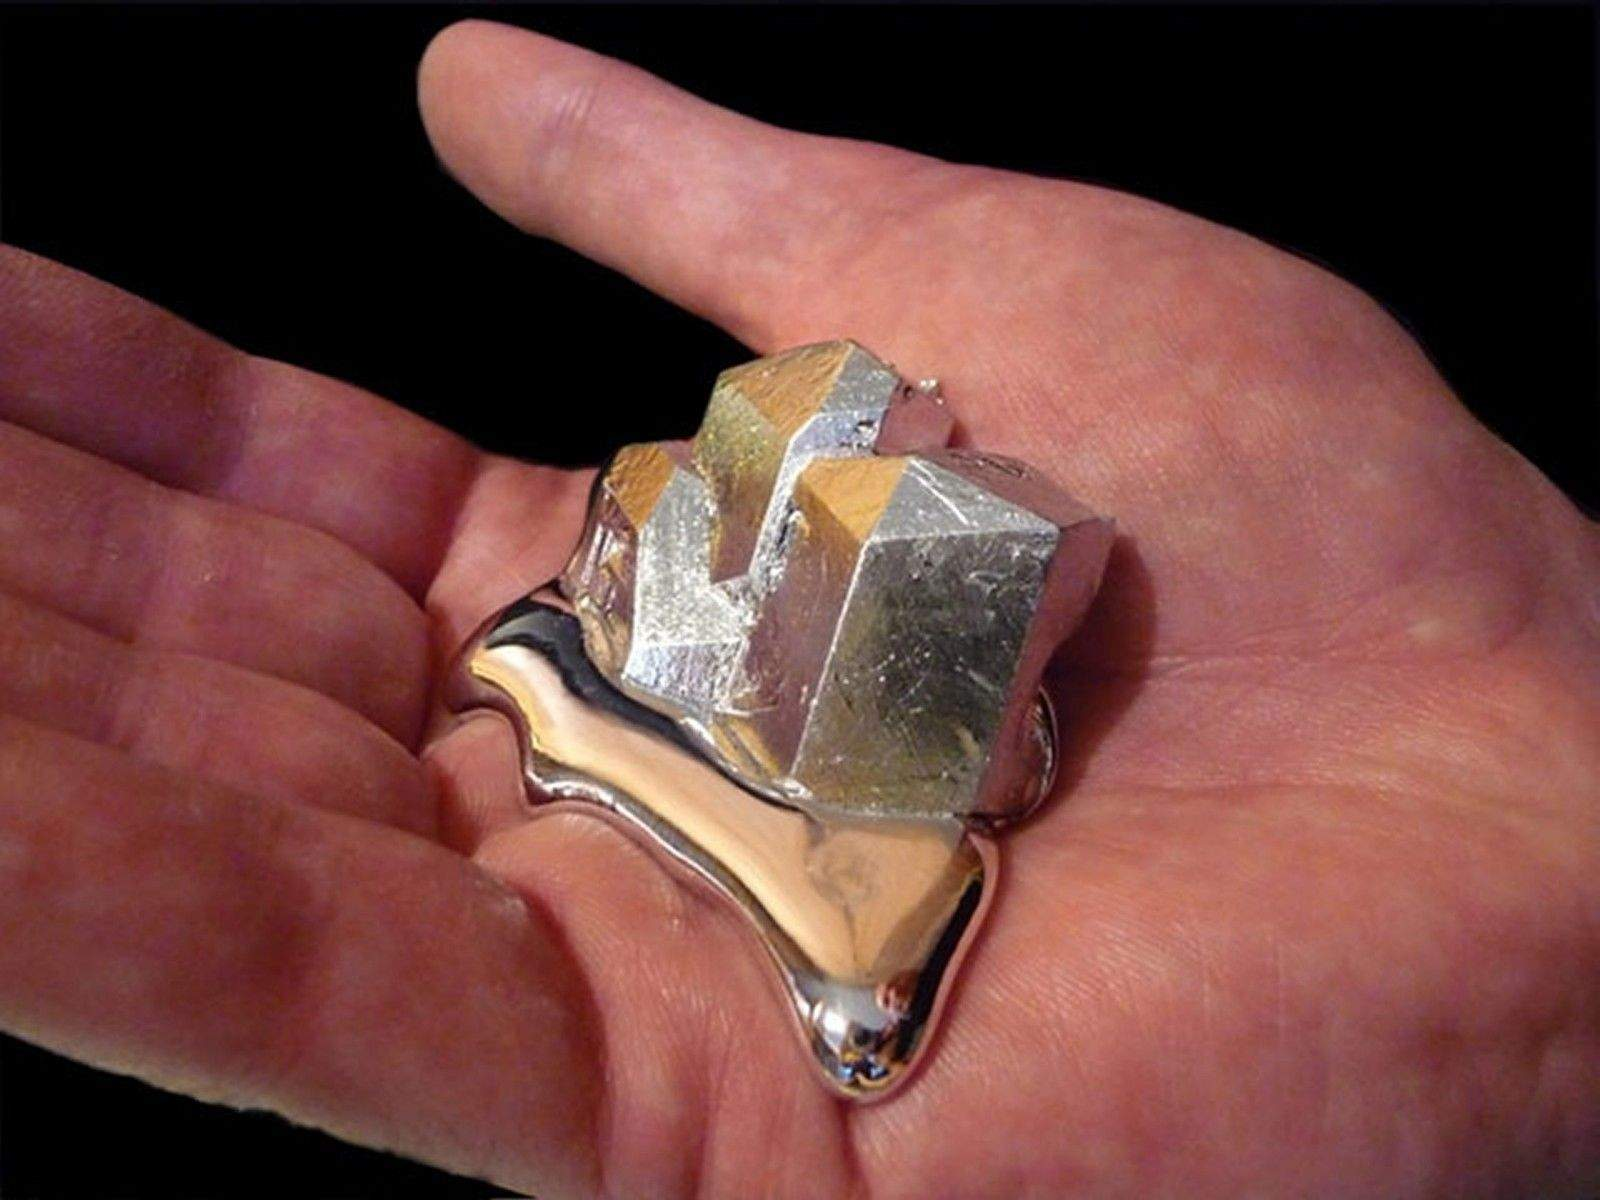
\includegraphics[width=\textwidth]{gálio.png}
    \\
    \vspace{2cm}
    \textbf{Uniacademia , Juiz De Fora, Minas Gerais}
    
\end{center}
\newpage
\tableofcontents
\newpage
\listoffigures
\newpage

\pagenumbering{arabic}
\nocite{*}
\section{Introdução}
O gálio no resfriamento de processadores é um avanço muito importante para solucionar a grande demanda por poder de processamento eficiente e sustentável. Com a evolução rápida da tecnologia, principalmente em áreas como jogos,inteligência artificial, análise de dados em tempo real e computação de alta performance em alta resolução,a cada ano que se passa é exigido cada vez mais um desempenho melhor e mais eficiente de um processador. 
Com isso, é necessária cada vez mais a criação de tecnologias de dissipação de calor de maneira mais eficaz. O calor excessivo em um processador não só limita seu desempenho, como também reduz sua vida útil, impactando diretamente a eficiência e a durabilidade dos componentes do hardware. É nesse contexto que o gálio surge como uma das opções promissoras para substituir ou complementar as soluções tradicionais de resfriamento, como pastas térmicas e resfriadores líquidos.
\begin{adjustbox}{center,caption={Placa Mãe do PS5 (Imagem: PlayStation/Reprodução)},nofloat=figure,vspace=\bigskipamount}
    \centering
    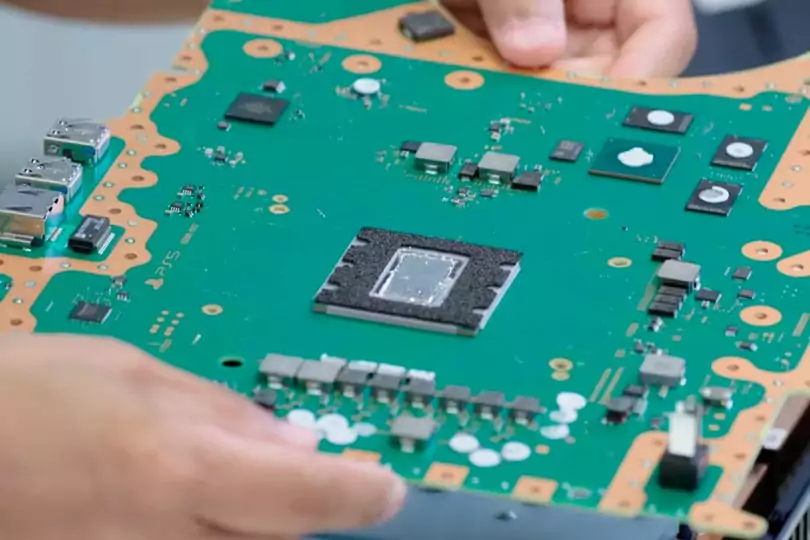
\includegraphics[width=12cm]{mobo.png}
\end{adjustbox}
Historicamente, a dissipação de calor sempre foi preocupante para a indústria de semicondutores. Com o aumento da densidade de transistores em chips, iniciado pela Lei de Moore nos anos 1960, a quantidade de calor gerada dentro de processadores aumentou proporcionalmente, tornando o gerenciamento térmico uma prioridade. Na década de 1990, com o surgimento dos primeiros processadores de alta performance, o uso de pastas térmicas se tornou um método muito adotado para otimizar a condução de calor entre o processador e o dissipador. 
No entanto, as pastas térmicas mais comuns possuem limitações, especialmente em relação à sua condutividade térmica, o que torna difícil acompanhar a demanda dos processadores modernos, cujas taxas de dissipação de calor já ultrapassam os 200 W.
O gálio, por ser um metal líquido, possui características que permitem ultrapassar os limites dos materiais convencionais, trazendo várias vantagens. Primeiramente,A condutividade térmica do gálio é significativamente superior à das pastas térmicas convencionais, proporcionando uma transferência de calor mais eficaz. Além disso, o ponto de fusão do gálio é de aproximadamente 29,76 °C, o que o faz líquido à temperatura ambiente em condições controladas, permitindo que ele preencha totalmente os espaços necessários entre o processador e o dissipador de calor. Essa capacidade de preencher imperfeições resulta em uma área de contato muito maior, melhorando substancialmente a eficiência de transferência térmica.
O uso do gálio em sistemas de resfriamento foi impulsionada pelos desenvolvimentos nas ligas de gálio, como o EGaIn (liga de gálio, índio e estanho), que une o alto desempenho térmico com maior estabilidade química. Essas ligas apresentam uma grande resistência à evaporação e à degradação ao longo do tempo, além de possuírem propriedades de molhabilidade (habilidade de se fixar facilmente em superfícies metálicas), ampliando o contato térmico e a eficiência na dissipação de calor. Assim, o uso de gálio ou de ligas de gálio pode reduzir significativamente a temperatura de operação de um processador, possibilitando clocks (velocidade com que ele executa suas operações, ou seja, o número de ciclos que o chip realiza por segundo) mais altos e desempenho otimizado sem superaquecimento.
Porém, o uso de gálio em sistemas de resfriamento de processadores não está isento de problemas. O gálio tem um comportamento agressivo em relação a certos metais, como o alumínio, corroendo esses materiais com o passar do tempo. Essa corrosão acontece por causa da elevada reatividade do gálio, que tem a capacidade de penetrar nas camadas superficiais de metais vulneráveis, prejudicando a integridade estrutural do dissipador ou até mesmo do processador. Esse problema ocorre somente quando o gálio é utilizado puro e exige o desenvolvimento de ligas e soluções de isolamento que sejam compatíveis com os materiais utilizados nos sistemas de resfriamento.
Dessa forma, o objetivo deste estudo é explorar as aplicações do gálio no resfriamento de processadores, mostrando os benefícios, limitações e inovações técnicas necessárias para integrar esse material de forma segura e eficaz. Além de avaliar as possibilidades de resfriamento mais eficientes, buscamos entender como a indústria está lidando com os problemas impostos pelo gálio, visando uma aplicação mais abrangente e sustentável em grande escala.
\section{Revisão de Literatura}
\subsection{História do gálio}
O gálio foi descoberto em Paris por Paul-Émile Lecoq de Boisbaudran em 1875. Ele observou uma nova linha violeta no espectro atômico de zinco extraído de uma amostra de blenda de zinco (ZnS) dos Pirineus, o que indicava a presença de um elemento desconhecido.
Boisbaudran não sabia que Dmitri Mendeleev já havia previsto a existência e propriedades desse elemento, sugerindo uma massa atômica de 68 e densidade de 5,9 g/cm³. Em novembro de 1875, Boisbaudran isolou e purificou o metal, apresentando-o à Academia Francesa de Ciências em dezembro.
\subsubsection{Onde podemos encontrá lo no planeta:}
O Gálio é encontrado em minérios de alumínio e zinco, como a bauxita e a blenda de zinco (ZnS), geralmente como um subproduto da mineração desses elementos. no Brasil, ele pode ser extraído em depósitos de bauxita, como em Minas Gerais, que é um grande produtor de alumínio.
\subsubsection{Processo de Extração}
A extração do Gálio ocorre durante o processo da bauxita, onde se acumula em soluções alcalinas. Essas soluções passam por um processo de eletrodeposição (processo eletroquímico que consiste em revestir uma peça metálica com outro material através da aplicação de corrente elétrica) para recuperar o gálio, que é purificado posteriormente. 
\section{Como funciona o resfriamento de um computador}
A eficiência e o desempenho de um PC estão diretamente relacionados à sua capacidade de gerenciar o calor,sem um controle eficaz da temperatura, o excesso de calor pode reduzir a longevidade dos componentes, afetar o desempenho e, em casos extremos, causar danos irreparáveis. É justamente que entram os conceitos de resfriamento
Resfriamento em PCs geralmente se refere ao uso de ar (imagem 2) ou líquido (imagem 3) para remover o excesso de calor dos componentes, utilizando ventiladores, dissipadores de calor ou sistemas de refrigeração líquida.
\begin{adjustbox}{center,caption={Air Cooler de computador em detalhe},nofloat=figure,vspace=\bigskipamount}
    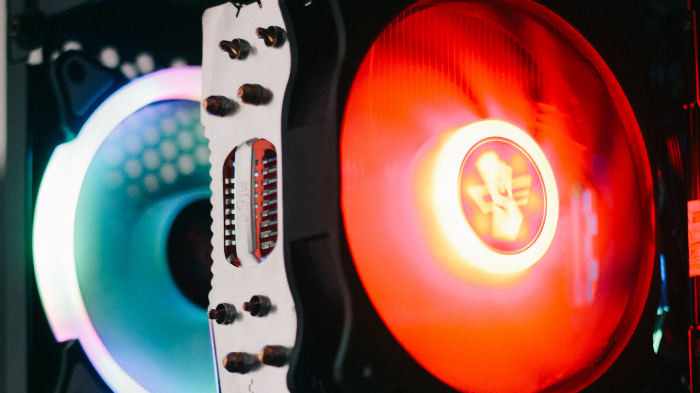
\includegraphics[width=8cm]{cooler.png}

\end{adjustbox}
\begin{adjustbox}{center,caption={Computador Gamer que utiliza refrigeração liquida},nofloat=figure,vspace=\bigskipamount}
    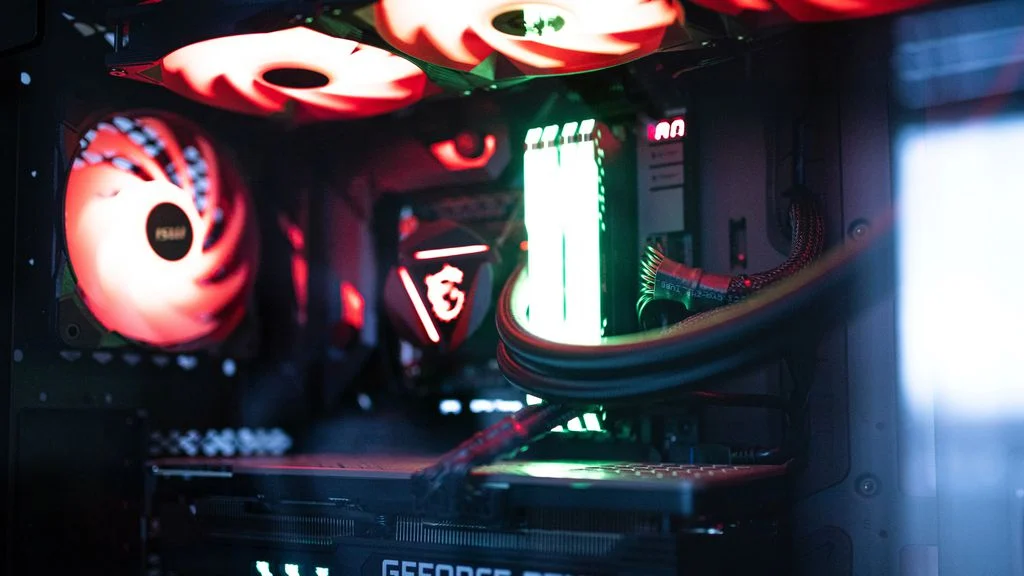
\includegraphics[width=12cm]{gaymer.png}
\end{adjustbox}{center}
Os sistemas de resfriamento são necessários para manter a temperatura dos componentes do PC dentro de limites seguros, garantindo desempenho e estabilidade. Existem dois métodos principais de resfriamento: a ar e líquido, cada um com suas vantagens e desvantagens.
\subsection{Refrigeração à ar}
O resfriamento a ar é o método mais comum e acessível de manter os componentes do PC frios. Ele utiliza ventiladores (coolers) para mover o ar através de dissipadores de calor, que são projetados para aumentar a área de superfície para dissipação eficiente do calor. Este método é eficaz para a maioria dos PCs de uso geral e jogos de nível de entrada a médio.
\begin{adjustbox}{center,caption={Funcionamento básico de refrigeração a ar (Imagem: Intel/Divulgação)},nofloat=figure,vspace=\bigskipamount}
    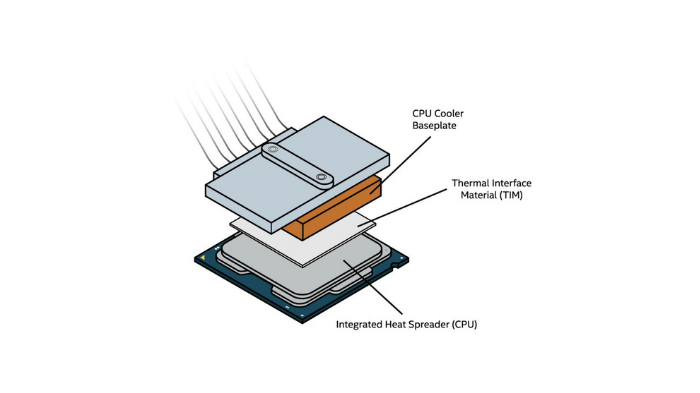
\includegraphics[width=12cm]{fusca.png}
\end{adjustbox}
\subsection{Refrigeração à agua}
á este método utiliza um líquido refrigerante para absorver e dissipar o calor dos componentes do PC. O líquido é circulado através de blocos de resfriamento acoplados aos componentes e depois resfriado em um radiador. Ele é mais eficiente termicamente e é preferido para overclocking e sistemas de alta performance.
\begin{adjustbox}{center,caption={Exemplo de refrigeração liquida (Imagem: Intel/Divulgação)},nofloat=figure,vspace=\bigskipamount}
    \includegraphics[width=12cm]{ap.png}
\end{adjustbox}
\section{Utilização do gálio no sistema de resfriamento de computadores}
O gálio é um metal raro, com características únicas que o tornam ideal para o gerenciamento térmico em eletrônica de alta densidade. Entre suas principais propriedades está o baixo ponto de fusão, aproximadamente 29,76 °C, o que permite que ele permaneça em estado líquido em condições de operação normais. Esse estado líquido facilita a "molhabilidade" do gálio, ou seja, sua capacidade de se espalhar e cobrir superfícies metálicas de forma uniforme, o que maximiza a área de contato para transferência de calor (Chiu \\\\\& Xiao).
Um dos grandes benefícios do gálio como material térmico é sua condutividade térmica, que é substancialmente superior às pastas térmicas comuns. Essa propriedade é essencial para processadores que operam em alta carga e geram grande quantidade de calor. A liga EGaIn, por exemplo, permite que o calor seja rapidamente transferido para o dissipador, evitando o superaquecimento e aumentando o desempenho do processador. (Pereira \& Souza).
\begin{adjustbox}{center,caption={Grafico Comparativo entre Pasta térmica e Metal liquido (Imagem: Tom's Hardware)},nofloat=figure,vspace=\bigskipamount}
    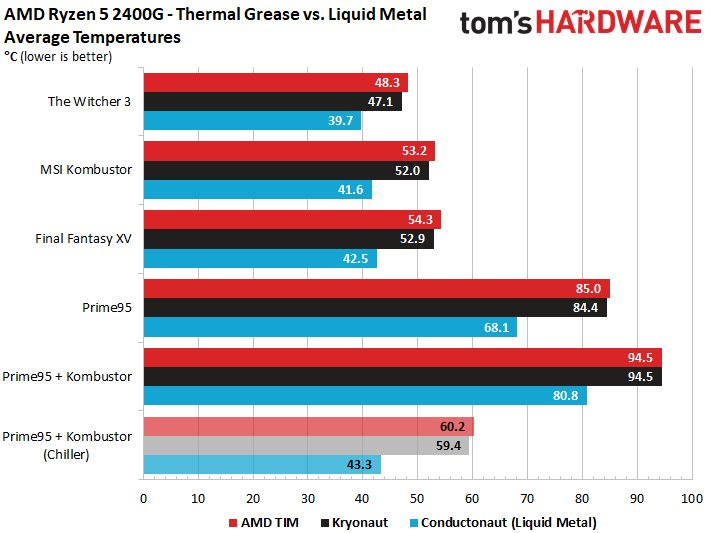
\includegraphics[width=15cm]{tio_hardware.jpg}
\end{adjustbox}
O gráfico apresentado pela Tom's Hardware (imagem 1) compara a eficiência de diferentes compostos térmicos na dissipação de calor de um processador AMD Ryzen 5 2400G. 
As substâncias testadas foram:
AMD TIM: A pasta térmica padrão que acompanha o processador.
Kryonaut: Uma pasta térmica de alta performance.
Conductonaut (Metal liquido): Uma liga metálica, à base de gálio, que é considerada uma das melhores opções para dissipação de calor.
Gálio (Conductonaut) se destaca: Em quase todos os testes, o Conductonaut apresentou as temperaturas mais baixas, indicando uma dissipação de calor significativamente melhor em comparação com as pastas térmicas.
A pasta térmica Kryonaut também apresentou bons resultados, ficando em segundo lugar na maioria dos testes.
AMD TIM é a menos eficiente: A pasta térmica padrão da AMD apresentou as temperaturas mais altas, demonstrando que não é a melhor opção para quem busca o máximo desempenho térmico.
Gálio sob carga extrema: Nos testes mais exigentes, como Prime95 + Kombustor, o gálio continuou mostrando superioridade, indicando que ele é capaz de manter o processador mais frio mesmo sob cargas de trabalho extremas.
Essas propriedades combinadas resultam em temperaturas de operação mais baixas para os componentes eletrônicos, aumentando sua vida útil e desempenho.
\section{Como funciona um console de Video Game e o porquê da utilização do Gálio como resfriamento}
O sistema de resfriamento do PS5 é sofisticado e combina metal líquido e uma câmara de vapor para manter o processador em uma temperatura ideal durante o uso intensivo. O metal líquido, feito de uma liga de gálio e índio, é colocado entre o processador e o dissipador de calor e atua como um condutor extremamente eficiente devido à sua elevada condutividade térmica.
De acordo com a Sony, o uso de metal líquido garantirá um desempenho de resfriamento “alto, estável e duradouro” no PlayStation 5. Segundo ressalta o Tweaktown, a solução entrega resultados até 86\% melhores que a pasta térmica convencional no PC.
\begin{adjustbox}{center,caption={O metal líquido garante melhor desempenho em comparação à pasta térmica. (Imagem: PlayStation/Reprodução)},nofloat=figure,vspace=\bigskipamount}
    \centering
    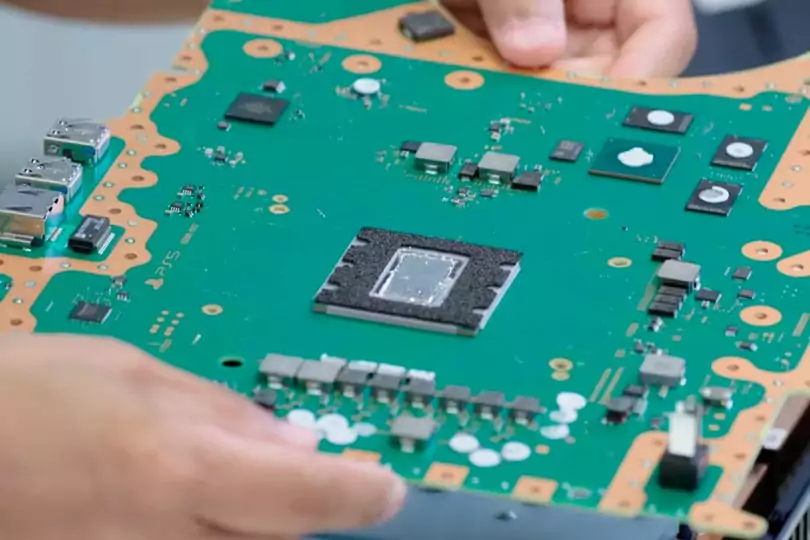
\includegraphics[width=12cm]{mobo.png}
\end{adjustbox}
\begin{itemize}
    \item \textbf{Condutividade Térmica Elevada:} A capacidade de transferir calor do metal líquido é cerca de cinco vezes maior do que a pasta térmica comum. Isso significa que ele pode extrair o calor do processador de forma rápida e transferi-lo ao dissipador, ajudando a evitar que o processador atinja temperaturas que possam reduzir seu desempenho.
    \item \textbf{Baixa Resistência Térmica:} O metal líquido forma uma camada extremamente fina entre o processador e o dissipador, o que reduz a resistência térmica. A resistência térmica baixa significa que o calor não encontra barreiras significativas ao sair do processador.
\end{itemize}
\subsection{Câmara de Vapor}
Após o metal líquido transferir o calor para o dissipador, a câmara de vapor entra em ação para redistribuir o calor de maneira uniforme. A câmara de vapor é uma estrutura selada que contém um fluido que evapora ao entrar em contato com o calor.
\begin{itemize}
    \item \textbf{Distribuição Uniforme:} Quando o fluido dentro da câmara de vapor se aquece, ele evapora e transporta o calor para outras áreas da câmara. Isso permite que o calor seja distribuído e dissipado de forma mais eficaz, evitando pontos quentes localizados que poderiam danificar componentes internos.
    \item \textbf{Eficiência no Resfriamento:} Como o vapor se condensa nas áreas mais frias da câmara, ele volta ao estado líquido e reinicia o ciclo, mantendo o sistema de resfriamento em funcionamento contínuo.
\end{itemize}
\begin{adjustbox}{center,caption={heatsink com cilindro dissipador que traz uma cobertura maior em relação ao modelo utilizado no PS4.},nofloat=figure,vspace=\bigskipamount}
    \centering
    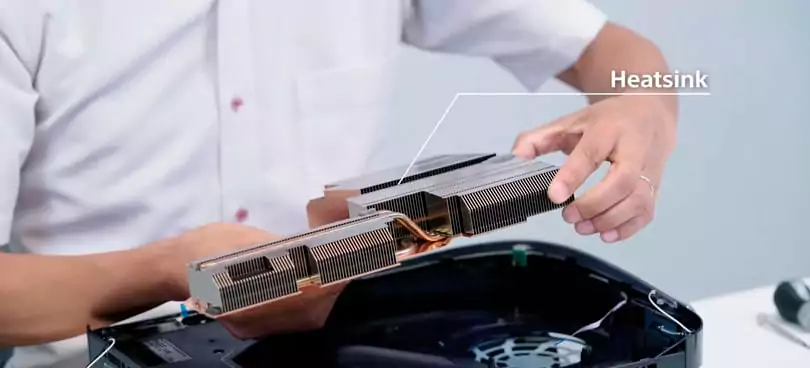
\includegraphics[width=12cm]{a_big_sink.png}
\end{adjustbox}
\subsection{Dispersão do Calor pelo Ventilador}
último estágio do processo de resfriamento é a dispersão do calor através do ventilador do PS5. O calor transferido do processador e redistribuído pela câmara de vapor é finalmente liberado para fora do console por meio de um fluxo de ar.
\begin{itemize}
    \item \textbf{Redução de Ruído: } Com o metal líquido e a câmara de vapor sendo altamente eficientes, o ventilador precisa trabalhar menos para manter as temperaturas estáveis, o que reduz o ruído produzido durante a operação
    \item \textbf{Controle Térmico Inteligente:}  A temperatura é monitorada e ajustada pelo sistema do PS5, que controla a velocidade do ventilador para otimizar o resfriamento conforme a demanda do processador.
\end{itemize}
\begin{adjustbox}{center,caption={Fan utilizada no playstation 5 (Imagem: PlayStation/Reprodução)},nofloat=figure,vspace=\bigskipamount}
    \centering
    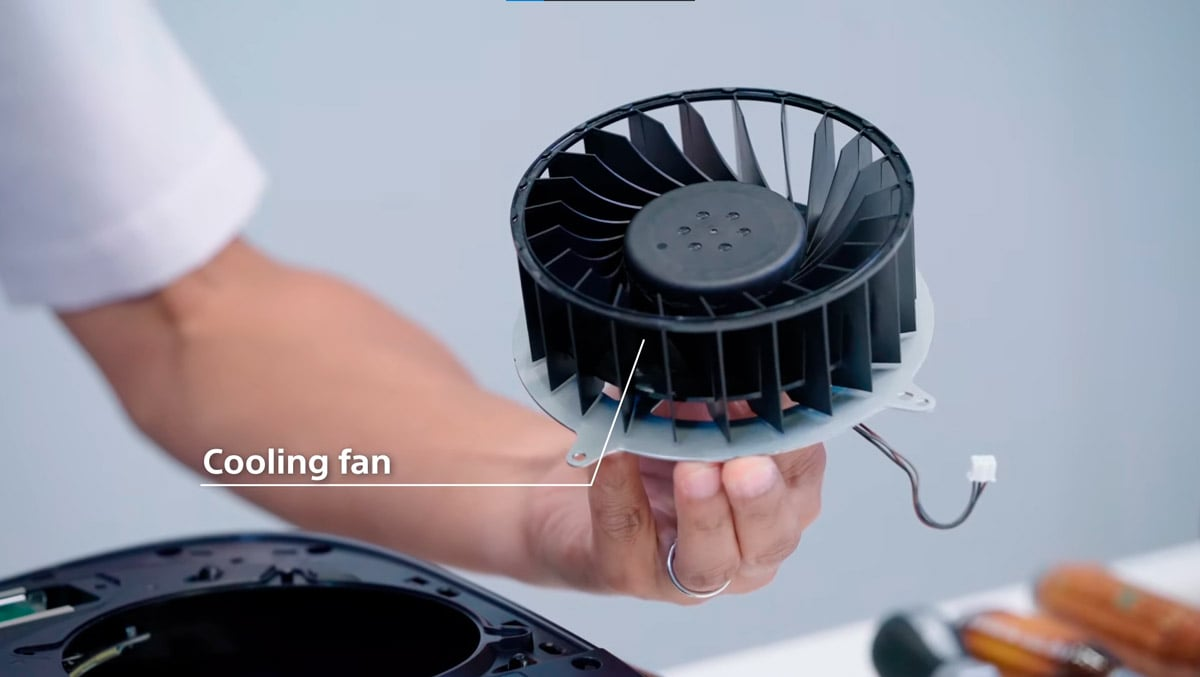
\includegraphics[width=12cm]{ventoinha.png}
\end{adjustbox}
\subsection{ Por Que o Metal Líquido é o mais recomendado?}
Comparado com a pasta térmica, o metal líquido é mais eficiente para manter temperaturas baixas em componentes de alto desempenho como o processador do PS5. Em condições de uso intenso, a pasta térmica tradicional chega a limitar a eficiência do resfriamento, pois ela tem menor capacidade de conduzir o calor.
\subsection{Testes práticos comparando PS5 com pasta térmica e Metal Liquido
Exemplos de Dados no Vídeo}
\begin{itemize}
    \item \textbf{Temperatura com Metal Líquido: } Em uso intenso, a temperatura média do processador com metal líquido fica em torno de 52°C.
    \item \textbf{emperatura com Pasta Térmica Tradicional: } Usando pasta térmica, o processador pode atingir até 65°C, um aumento que impacta a performance e a durabilidade do componente.
\end{itemize}
Portanto, o metal líquido permite ao PS5 manter seu desempenho máximo por mais tempo, e com menor risco de sobreaquecimento, sendo ideal para cenários de uso prolongado e exigente como em jogos de última geração.
\section{Riscos da utilização do Gálio e consequentemente do metal líquido}
\begin{adjustbox}{center,caption={Dissipador de calor que utiliza metal liquido},nofloat=figure,vspace=\bigskipamount}
    \centering
    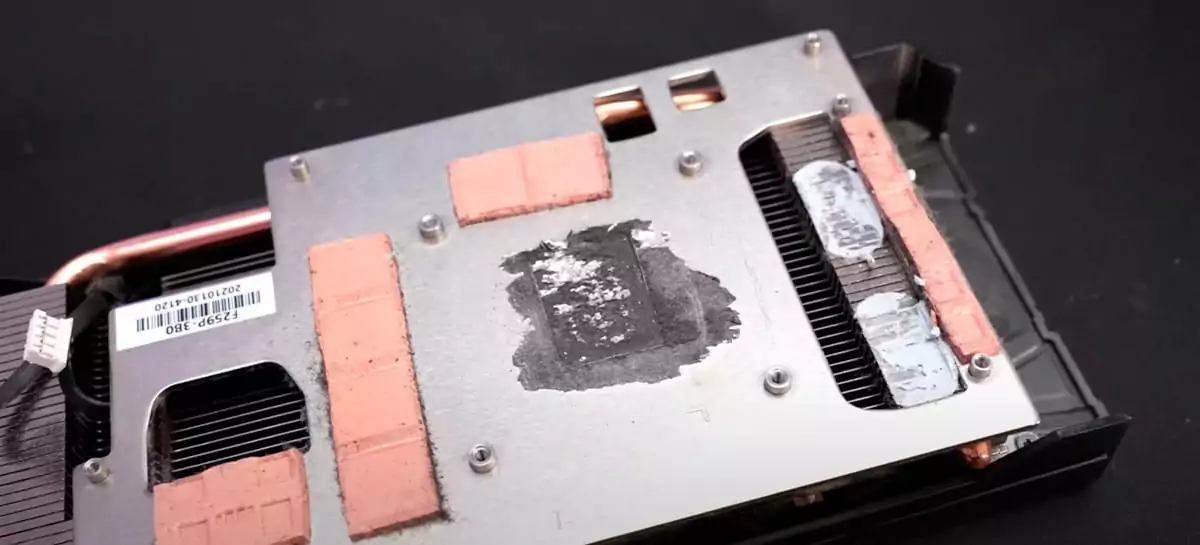
\includegraphics[width=12cm]{heatspreader.png}
\end{adjustbox}
\section{Evolução das Ligas Metálicas Líquidas na Dissipação Térmica}
A pesquisa com ligas metálicas líquidas para dissipação térmica começou a ganhar espaço nas últimas décadas, à medida que os limites das pastas térmicas convencionais se tornaram evidentes. A liga EGaIn, composta por gálio, índio e estanho, foi desenvolvida para combinar a alta condutividade térmica do gálio com a estabilidade química proporcionada pelo índio e pelo estanho, ampliando o uso do gálio em eletrônica de alta potência (Carvalho \& Lopes).
Além de oferecer vantagens em termos de condutividade térmica, essas ligas líquidas se destacam por sua durabilidade e resistência à evaporação. Diferente das pastas térmicas convencionais, que podem secar e perder eficiência ao longo do tempo, ligas como o EGaIn mantêm suas propriedades por períodos prolongados, aumentando a vida útil dos componentes eletrônicos. Estudos mostram que o uso de ligas metálicas líquidas de gálio pode reduzir as temperaturas operacionais dos processadores em até 15°C quando comparado com métodos convencionais (Oh et al).
\begin{adjustbox}{center,caption={Chip que utiliza metal liquido como interface termica},nofloat=figure,vspace=\bigskipamount}
    \centering
    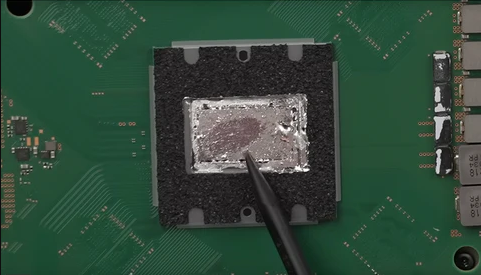
\includegraphics[width=12cm]{chip.png}
\end{adjustbox}
\section{Perspectivas Futuras e Conclusão sobre Materiais Térmicos}
O futuro do desenvolvimento de materiais térmicos para eletrônica de alta densidade parece promissor, especialmente no que diz respeito ao uso de gálio e suas ligas. A pesquisa continua focada em melhorar a estabilidade e a segurança das ligas metálicas líquidas, explorando a combinação de gálio com novos materiais e técnicas de encapsulamento para resolver os problemas de corrosão e compatibilidade. Segundo Almeida \& Ferreira, é possível que novos métodos de fabricação tornem o gálio mais acessível economicamente e aplicável em uma variedade de dispositivos, indo além dos processadores de alto desempenho para integrar-se também em sistemas de resfriamento de servidores e equipamentos de computação de larga escala.
À medida que a indústria de semicondutores evolui, a inovação em materiais térmicos será essencial para garantir a eficiência e a durabilidade dos dispositivos. Soluções como a liga EGaIn já demonstram um grande potencial e continuam a inspirar pesquisas. Para o Brasil, a introdução de materiais térmicos avançados abre portas para a modernização do setor tecnológico, criando um impacto positivo tanto na indústria quanto na academia (Pereira \& Souza).
\newpage
\printbibliography
\end{document}